%\iffalse
\let\negmedspace\undefined
\let\negthickspace\undefined
\documentclass[journal,12pt,twocolumn]{IEEEtran}
\usepackage{cite}
\usepackage{amsmath,amssymb,amsfonts,amsthm}
\usepackage{algorithmic}
\usepackage{graphicx}
\usepackage{textcomp}
\usepackage{xcolor}
\usepackage{txfonts}
\usepackage{listings}
\usepackage{enumitem}
\usepackage{mathtools}
\usepackage{gensymb}
\usepackage[breaklinks=true]{hyperref}
\usepackage{tkz-euclide} % loads  TikZ and tkz-base
\usepackage{listings}



\newtheorem{theorem}{Theorem}[section]
\newtheorem{problem}{Problem}
\newtheorem{proposition}{Proposition}[section]
\newtheorem{lemma}{Lemma}[section]
\newtheorem{corollary}[theorem]{Corollary}
\newtheorem{example}{Example}[section]
\newtheorem{definition}[problem]{Definition}
%\newtheorem{thm}{Theorem}[section] 
%\newtheorem{defn}[thm]{Definition}
%\newtheorem{algorithm}{Algorithm}[section]
%\newtheorem{cor}{Corollary}
\newcommand{\BEQA}{\begin{eqnarray}}
\newcommand{\EEQA}{\end{eqnarray}}
\newcommand{\define}{\stackrel{\triangle}{=}}
\theoremstyle{remark}
\newtheorem{rem}{Remark}
%\bibliographystyle{ieeetr}
\begin{document}
%
\providecommand{\pr}[1]{\ensuremath{\Pr\left(#1\right)}}
\providecommand{\prt}[2]{\ensuremath{p_{#1}^{\left(#2\right)} }}        % own macro for this question
\providecommand{\qfunc}[1]{\ensuremath{Q\left(#1\right)}}
\providecommand{\sbrak}[1]{\ensuremath{{}\left[#1\right]}}
\providecommand{\lsbrak}[1]{\ensuremath{{}\left[#1\right.}}
\providecommand{\rsbrak}[1]{\ensuremath{{}\left.#1\right]}}
\providecommand{\brak}[1]{\ensuremath{\left(#1\right)}}
\providecommand{\lbrak}[1]{\ensuremath{\left(#1\right.}}
\providecommand{\rbrak}[1]{\ensuremath{\left.#1\right)}}
\providecommand{\cbrak}[1]{\ensuremath{\left\{#1\right\}}}
\providecommand{\lcbrak}[1]{\ensuremath{\left\{#1\right.}}
\providecommand{\rcbrak}[1]{\ensuremath{\left.#1\right\}}}
\newcommand{\sgn}{\mathop{\mathrm{sgn}}}
\providecommand{\abs}[1]{\left\vert#1\right\vert}
\providecommand{\res}[1]{\Res\displaylimits_{#1}} 
\providecommand{\norm}[1]{\left\lVert#1\right\rVert}
%\providecommand{\norm}[1]{\lVert#1\rVert}
\providecommand{\mtx}[1]{\mathbf{#1}}
\providecommand{\mean}[1]{E\left[ #1 \right]}
\providecommand{\cond}[2]{#1\middle|#2}
\providecommand{\fourier}{\overset{\mathcal{F}}{ \rightleftharpoons}}
\newenvironment{amatrix}[1]{%
  \left(\begin{array}{@{}*{#1}{c}|c@{}}
}{%
  \end{array}\right)
}
%\providecommand{\hilbert}{\overset{\mathcal{H}}{ \rightleftharpoons}}
%\providecommand{\system}{\overset{\mathcal{H}}{ \longleftrightarrow}}
	%\newcommand{\solution}[2]{\textbf{Solution:}{#1}}
\newcommand{\solution}{\noindent \textbf{Solution: }}
\newcommand{\cosec}{\,\text{cosec}\,}
\providecommand{\dec}[2]{\ensuremath{\overset{#1}{\underset{#2}{\gtrless}}}}
\newcommand{\myvec}[1]{\ensuremath{\begin{pmatrix}#1\end{pmatrix}}}
\newcommand{\mydet}[1]{\ensuremath{\begin{vmatrix}#1\end{vmatrix}}}
\newcommand{\myaugvec}[2]{\ensuremath{\begin{amatrix}{#1}#2\end{amatrix}}}
\providecommand{\rank}{\text{rank}}
\providecommand{\pr}[1]{\ensuremath{\Pr\left(#1\right)}}
\providecommand{\qfunc}[1]{\ensuremath{Q\left(#1\right)}}
	\newcommand*{\permcomb}[4][0mu]{{{}^{#3}\mkern#1#2_{#4}}}
\newcommand*{\perm}[1][-3mu]{\permcomb[#1]{P}}
\newcommand*{\comb}[1][-1mu]{\permcomb[#1]{C}}
\providecommand{\qfunc}[1]{\ensuremath{Q\left(#1\right)}}
\providecommand{\gauss}[2]{\mathcal{N}\ensuremath{\left(#1,#2\right)}}
\providecommand{\diff}[2]{\ensuremath{\frac{d{#1}}{d{#2}}}}
\providecommand{\myceil}[1]{\left \lceil #1 \right \rceil }
\newcommand\figref{Fig.~\ref}
\newcommand\tabref{Table~\ref}
\newcommand{\sinc}{\,\text{sinc}\,}
\newcommand{\rect}{\,\text{rect}\,}
%%
%	%\newcommand{\solution}[2]{\textbf{Solution:}{#1}}
%\newcommand{\solution}{\noindent \textbf{Solution: }}
%\newcommand{\cosec}{\,\text{cosec}\,}
%\numberwithin{equation}{section}
%\numberwithin{equation}{subsection}
%\numberwithin{problem}{section}
%\numberwithin{definition}{section}
%\makeatletter
%\@addtoreset{figure}{problem}
%\makeatother

%\let\StandardTheFigure\thefigure
\let\vec\mathbf

\bibliographystyle{IEEEtran}


\vspace{3cm}



\bigskip

\renewcommand{\thefigure}{\theenumi}
\renewcommand{\thetable}{\theenumi}
%\renewcommand{\theequation}{\theenumi}
Question  An urn contains 25 balls of which 10 balls bear a mark $X$ and the remaining 15 bear a mark $Y$. A ball is drawn at random from the urn, its mark is noted down and it is replaced. If 6 balls are drawn in this way, find the probability that\\
\begin{enumerate}
\item all will bear $X$ mark.\\
\item not more than 2 will bear $Y$ mark.\\
\item at least one ball will bear $Y$ mark.\\
\item the number of balls with X mark and $Y$ mark will be equal.\\
\end{enumerate}
\solution  \\
\begin{enumerate}
\begin{table}[!ht]
\centering
\begin{tabular}{|l|c|r|}
    \hline
    Parameter & Values & Description\\
    \hline
    $n$ & 6 & Number of draws\\
    \hline
    $p$ & 0.4 & Probability that ball bears $X$ mark \\
    \hline
    $q$ & 0.6 & Probability that ball bears $X$ mark \\
    \hline
    $\mu$ & 2.4 & $np$ \\
    \hline
    $\sigma $ & 1.2 & $\sqrt{np(1 - p)} $\\
    \hline
\end{tabular}
\caption{Definition of parameters}
\label{tab:gaussian/9/3/17}
\end{table}
\item all will bear '$X$ mark
We know that Q-function is given as
\begin{align}
Q(x) &= \pr{X > x}
\end{align}
Now, we want to find probability that all will bear $X$ mark.
\begin{align}
\pr{X = 0} &=1-\pr{X > 0} \\
&=1-\pr{\frac{X - \mu}{\sigma} > \frac{0 - 2.4}{1.2}} \\
&= 1- Q(-2)\\
&= 1- \int_{-2}^{\infty}\frac{1}{\sqrt{2\pi}}\times e^{-\frac{x^2}{2}}dx\\
&= 1-0.9958\\
&=0.004082
\end{align}
\textbf{Binomial}
\begin{align}
\pr{X =0} &= 1 - \pr{X> 0} \\
&= \comb{n}{k}p^k\brak{1-p}^{n-k} \\
&= 0.004096
\end{align}
\item not more than 2 will bear $Y$ mark.\\
We know that Q-function is given as\\
\begin{align}
Q(x) &= \pr{X > x}\\
&= \int_{x}^{\infty}\frac{1}{\sqrt{2\pi}}\times e^{-\frac{x^2}{2}}dx
\end{align}
We need to find probability that not more than 2 will bear $Y$ mark
\begin{align}
\pr{X \leq 2} &= 1 - \pr{X > 2}\\
&= 1 - \pr{\frac{X - \mu}{\sigma} > \frac{2 - 3.6}{1.2}} \\
&= 1 - Q(-1.33)\\
&= 1 - \int_{-1.33}^{\infty}\frac{1}{\sqrt{2\pi}}\times e^{-\frac{x^2}{2}}dx\\
&= 1- 0.921\\
&=0.179
\end{align}
\textbf{Binomial}
\begin{align}
\pr{X\leq 2} &= 1 - \pr{X>2} \\
&= 1-\sum_{k=3}^{6} \comb{n}{k}p^k\brak{1-p}^{n-k} \\
&= 0.1792
\end{align}

\item at least one ball will bear $Y$ mark.\\
We know that Q-function is given as\\
\begin{align}
Q(x) &= \pr{X > x}
\end{align}
We need to find the probability that at least one ball will bear $Y$ mark.
\begin{align}
	\Pr(X \geq 1) &=\Pr(X > 0)\\
	&= \pr{\frac{X - \mu}{\sigma} > \frac{0 - 3.6}{\sqrt{1.2}}} \\
	&=\pr{\frac{X - \mu}{\sigma} > -3} \\
	&=0.99586\\
\end{align}
\textbf{Binomial}
\begin{align}
\pr{X\ge 1} &= 1 - \pr{X=0} \\
&= 1- \comb{n}{k}p^k\brak{1-p}^{n-k} \\
&=0.995904 
\end{align}
\item the number of balls with X mark and $Y$ mark will be equal.\\
Here, Probability that the number of balls with X mark and $Y$ mark will be equal.
\begin{align}
\pr{X = 3} &= 1 - Q(x)\\
 &= 1-\frac{X - \mu}{\sigma} \\
	&= 0.2763\\        
\end{align}
\end{enumerate}
\textbf{Binomial}
\begin{align}
\pr{X=3} 
&= \comb{n}{k}p^k\brak{1-p}^{n-k} \\
&= 0.2764
\end{align}
\begin{figure}
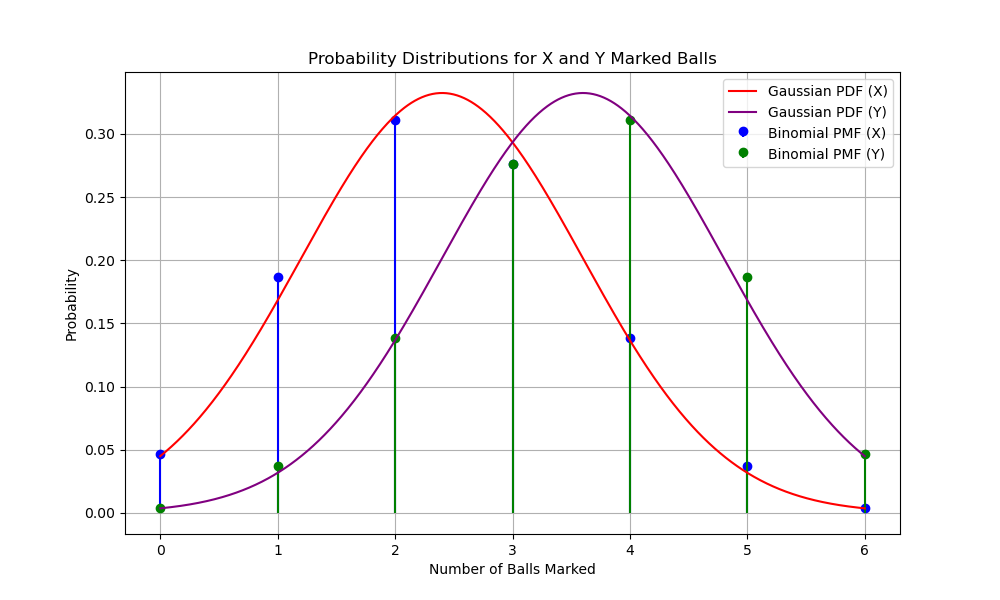
\includegraphics[width=\columnwidth]{/home/sravanthi/17/figs/Fig1.png}
\caption{pmf of binomial and pdf of Gaussian of X and Y marked balls}
\label{fig:gaussian/9/3/17/}
\end{figure}
\end{document}
